%
% LaTeX template for ICAP 2010 abstracts.
%
\documentclass[10pt]{article}

\usepackage{graphicx}
\usepackage{icap2010}

\begin{document}
%%%%%%%%%   DO NOT MODIFY ANYTHING ABOVE THIS LINE %%%%%%%%

\title{Ultranarrow dark resonance in caesium using mode-locked Ti:sapphire laser and buffer gas}

\begin{authors}
  \author{G.}{Imreh}{1},
  \author{T-H.}{Wu}{1},
  \author{C-M.}{Wu}{1},
  \author{Z-L.}{Yang}{1},
  \author{W-Y.}{Cheng}{1},
\end{authors}

\address{1}{Institute of Atomic and Molecular Sciences, Academia Sinica, Taiwan}

\begintext

Dark resonances due to coherent population trapping (CPT) offer naturally narrow linewiths and
are well suited for frequency standards. The width of these resonances can be reduced
by using high pressure buffer gas. In continous wave (CW) systems linewidth below 30Hz were
previously observed in rubidium\footnote{M.~Erhard and H.~Helm,``Buffer-gas effects on dark resonances: Theory and experiment'',
PRA {\bf 63}, 043813 (2001)}.

To further improve the resonance linewith we use a mode-locked Ti:saphire laser to provide the pump beams. This has the advantage that all interacting modes are in phase with each other, unlike the CW case where the phase coherence of the pump lasers limits the achiveable CPT performance. Our system is unique in that the repetition rate and the offset frequency can be tuned independently \footnote{W-Y.~Cheng, T-H.~Wu, S-W.~Huang, S-Y.~Lin and C-M.~Wu,``Stabilizing the frequency of femtosecond Ti:sapphire comb laser by a novel scheme'', Applied Physics B {\bf 92}, 13 (2008)}. 

The repetition rate of the mode-locked laser is set to be near an integer multiple of the ground state hyperfine splitting of caesium, and by scanning the repetition rate we can probe the dark resonance signal. In a cell buffered with 8700kPa neon at 100$^\circ$C we record 6.1(8)Hz linewidth. The large frequency shift of the resonance expected from the CW case due to teh buffer gas (several kHz) is not present, the observed shift is much less than the observed linewidth. The experiment was repeated in a cell buffered with a mixture of helium and nitrogen where only larger linewidth of 79(23)Hz were achiveable but still without the expected frequency shift. 

An optical clock based on CPT signal using mode locked lasers will have the advantage of narrower resonance, much reduced systematic frequency shifting effects, due to its higher peak power the ability to use thicker optical medium thus achieving better signal-to-noise ratio.

Our systematic studies of the this CPT signal and its theoretical analysis is presented.

\begin{center}
  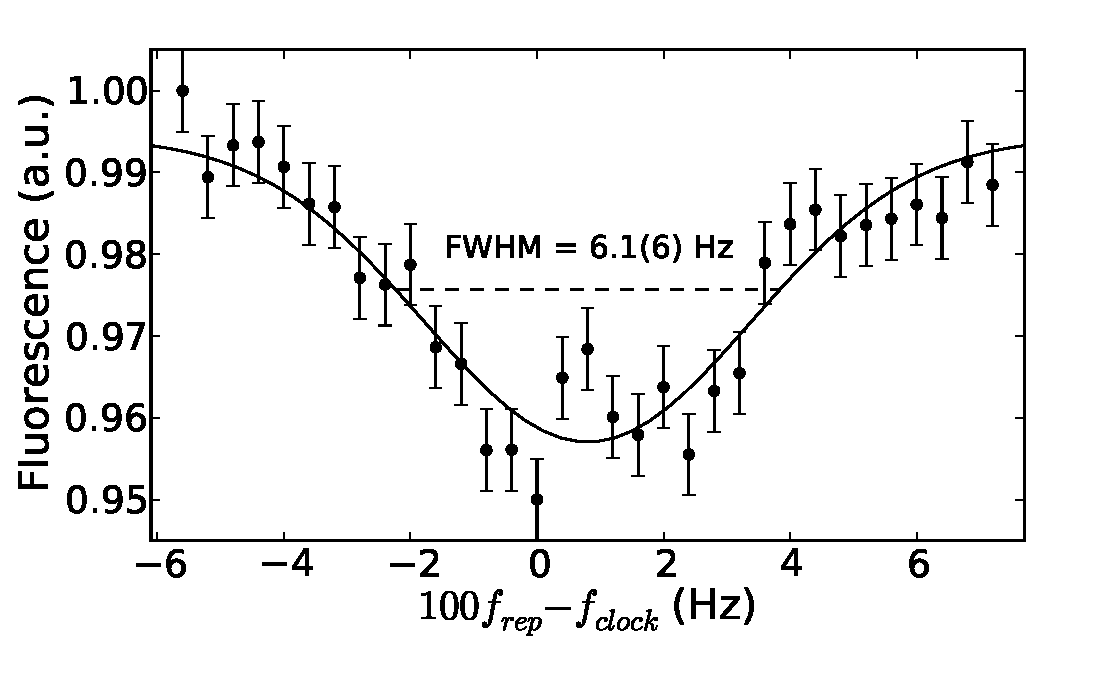
\includegraphics[width=0.6\textwidth]{8700Ne_buffer.eps}
\end{center}

%%%%%%%%%%   DO NOT MODIFY ANYTHING BELOW THIS LINE %%%%%%%%
\end{document}
